\documentclass[9pt,a4paper,]{extarticle}

\usepackage{f1000_styles}

\usepackage[pdfborder={0 0 0}]{hyperref}

\usepackage[numbers]{natbib}
\bibliographystyle{unsrtnat}


%% maxwidth is the original width if it is less than linewidth
%% otherwise use linewidth (to make sure the graphics do not exceed the margin)
\makeatletter
\def\maxwidth{ %
  \ifdim\Gin@nat@width>\linewidth
    \linewidth
  \else
    \Gin@nat@width
  \fi
}
\makeatother

\usepackage{color}
\usepackage{fancyvrb}
\newcommand{\VerbBar}{|}
\newcommand{\VERB}{\Verb[commandchars=\\\{\}]}
\DefineVerbatimEnvironment{Highlighting}{Verbatim}{commandchars=\\\{\}}
% Add ',fontsize=\small' for more characters per line
\usepackage{framed}
\definecolor{shadecolor}{RGB}{248,248,248}
\newenvironment{Shaded}{\begin{snugshade}}{\end{snugshade}}
\newcommand{\AlertTok}[1]{\textcolor[rgb]{0.94,0.16,0.16}{#1}}
\newcommand{\AnnotationTok}[1]{\textcolor[rgb]{0.56,0.35,0.01}{\textbf{\textit{#1}}}}
\newcommand{\AttributeTok}[1]{\textcolor[rgb]{0.77,0.63,0.00}{#1}}
\newcommand{\BaseNTok}[1]{\textcolor[rgb]{0.00,0.00,0.81}{#1}}
\newcommand{\BuiltInTok}[1]{#1}
\newcommand{\CharTok}[1]{\textcolor[rgb]{0.31,0.60,0.02}{#1}}
\newcommand{\CommentTok}[1]{\textcolor[rgb]{0.56,0.35,0.01}{\textit{#1}}}
\newcommand{\CommentVarTok}[1]{\textcolor[rgb]{0.56,0.35,0.01}{\textbf{\textit{#1}}}}
\newcommand{\ConstantTok}[1]{\textcolor[rgb]{0.00,0.00,0.00}{#1}}
\newcommand{\ControlFlowTok}[1]{\textcolor[rgb]{0.13,0.29,0.53}{\textbf{#1}}}
\newcommand{\DataTypeTok}[1]{\textcolor[rgb]{0.13,0.29,0.53}{#1}}
\newcommand{\DecValTok}[1]{\textcolor[rgb]{0.00,0.00,0.81}{#1}}
\newcommand{\DocumentationTok}[1]{\textcolor[rgb]{0.56,0.35,0.01}{\textbf{\textit{#1}}}}
\newcommand{\ErrorTok}[1]{\textcolor[rgb]{0.64,0.00,0.00}{\textbf{#1}}}
\newcommand{\ExtensionTok}[1]{#1}
\newcommand{\FloatTok}[1]{\textcolor[rgb]{0.00,0.00,0.81}{#1}}
\newcommand{\FunctionTok}[1]{\textcolor[rgb]{0.00,0.00,0.00}{#1}}
\newcommand{\ImportTok}[1]{#1}
\newcommand{\InformationTok}[1]{\textcolor[rgb]{0.56,0.35,0.01}{\textbf{\textit{#1}}}}
\newcommand{\KeywordTok}[1]{\textcolor[rgb]{0.13,0.29,0.53}{\textbf{#1}}}
\newcommand{\NormalTok}[1]{#1}
\newcommand{\OperatorTok}[1]{\textcolor[rgb]{0.81,0.36,0.00}{\textbf{#1}}}
\newcommand{\OtherTok}[1]{\textcolor[rgb]{0.56,0.35,0.01}{#1}}
\newcommand{\PreprocessorTok}[1]{\textcolor[rgb]{0.56,0.35,0.01}{\textit{#1}}}
\newcommand{\RegionMarkerTok}[1]{#1}
\newcommand{\SpecialCharTok}[1]{\textcolor[rgb]{0.00,0.00,0.00}{#1}}
\newcommand{\SpecialStringTok}[1]{\textcolor[rgb]{0.31,0.60,0.02}{#1}}
\newcommand{\StringTok}[1]{\textcolor[rgb]{0.31,0.60,0.02}{#1}}
\newcommand{\VariableTok}[1]{\textcolor[rgb]{0.00,0.00,0.00}{#1}}
\newcommand{\VerbatimStringTok}[1]{\textcolor[rgb]{0.31,0.60,0.02}{#1}}
\newcommand{\WarningTok}[1]{\textcolor[rgb]{0.56,0.35,0.01}{\textbf{\textit{#1}}}}

% disable code chunks background
%\renewenvironment{Shaded}{}{}

% disable section numbers
\setcounter{secnumdepth}{0}

%% added by MLS, this is not in the F1000 style by default %%

\hypersetup{unicode=true,
            pdftitle={BASiCS workflow: a step-by-step analysis of expression variability using single cell RNA sequencing data},
            pdfkeywords={Single-cell RNA sequencing, expression variability, transcriptional noise, differential expression testing},
            colorlinks=true,
            linkcolor=Maroon,
            citecolor=Blue,
            urlcolor=Orange,
            breaklinks=true}

%% End added by MLS %%

\setlength{\parindent}{0pt}
\setlength{\parskip}{6pt plus 2pt minus 1pt}



\begin{document}
\pagestyle{front}

\title{BASiCS workflow: a step-by-step analysis of expression variability using single cell RNA sequencing data}

\author[1]{Alan O'Callaghan\thanks{\ttfamily a.b.o'callaghan@sms.ed.ac.uk}}
\author[2]{Nils Eling}
\author[3,4]{John C. Marioni}
\author[1,5]{Catalina A. Vallejos\thanks{\ttfamily catalina.vallejos@igmm.ed.ac.uk}}
\affil[1]{MRC Human Genetics Unit, Institute of Genetics \& Molecular Medicine, University of Edinburgh, Western General Hospital, Crewe Road, Edinburgh, EH4 2XU, UK}
\affil[2]{Department of Quantitative Biomedicine, University of Zurich, Winterthurerstrasse 190, CH-8057, Zurich, Switzerland}
\affil[3]{European Molecular Biology Laboratory, European Bioinformatics Institute, Wellcome Trust Genome Campus, Hinxton, Cambridge CB10 1SD, UK}
\affil[4]{Cancer Research UK Cambridge Institute, University of Cambridge, Li Ka Shing Centre, Cambridge, CB2 0RE, UK}
\affil[5]{The Alan Turing Institute, British Library, 96 Euston Road, London, NW1 2DB, UK}

\maketitle
\thispagestyle{front}

\begin{abstract}
Cell-to-cell gene expression variability is an inherent feature of complex
biological systems, such as immunity and development. Single-cell RNA
sequencing is a powerful tool to quantify this heterogeneity, but it is prone
to strong technical noise. In this article, we describe a step-by-step
computational workflow that uses the BASiCS Bioconductor package to robustly
quantify expression variability within and between known groups of cells (such
as experimental conditions or cell types). BASiCS uses an integrated framework
for data normalisation, technical noise quantification and downstream
analyses, whilst propagating statistical uncertainty across these steps.
Within a single seemingly homogeneous cell population, BASiCS can identify
highly variable genes that exhibit strong heterogeneity as well as lowly
variable genes with stable expression. BASiCS also uses a probabilistic
decision rule to identify changes in expression variability between cell
populations, whilst avoiding confounding effects related to differences in
technical noise or in overall abundance. Using a publicly available
dataset, we guide users through a complete pipeline that includes
preliminary steps for quality control, as well as data exploration
using the scater and scran Bioconductor packages. Data for the case
study was generated using the Fluidigm@ C1 system, in which extrinsic
spike-in RNA molecules were added as a control. The workflow is accompanied
by a Docker image that ensures the reproducibility of our results.
\end{abstract}

\section*{Keywords}
Single-cell RNA sequencing, expression variability, transcriptional noise, differential expression testing


\clearpage
\pagestyle{main}

\hypertarget{introduction}{%
\section{Introduction}\label{introduction}}

Single-cell RNA-sequencing (scRNA-seq) enables the study of genome-wide
transcriptional heterogeneity in cell populations that is not
captured by bulk experiments \citep{Stegle2015, Prakadan2017, Patange2018}.
On the broadest level, this heterogeneity can reflect the presence of distinct
cell subtypes or states.
Alternatively, it can be due to gradual changes along biological processes,
such as development and differentiation.
Several clustering and pseudotime inference methods have been developed to
characterise these types of heterogeneity \citep{Kiselev2019, Saelens2019}.
However, there is a limited availability of computational tools tailored
to study more subtle variability within seemingly homogeneous cell populations.
This variability can reflect deterministic or stochastic events that regulate
gene expression and, among others, has been reported to increase prior to cell
fate decisions \citep{Mojtahedi2016} as well as during ageing \citep{Martinez-jimenez2017}.

Stochastic variability within a seemingly homogeneous cell population --- often
referred to as transcriptional \emph{noise} --- can arise from intrinsic and
extrinsic sources \citep{Elowitz2002, Eling2019}.
Extrinsic noise refers to stochastic fluctuations induced by
different dynamic cellular states (e.g.~cell cycle, metabolism,
intra/inter-cellular signalling) \citep{Zopf2013, Iwamoto2016, Kiviet2014}.
In contrast, intrinsic noise arises from stochastic effects on biochemical
processes such as transcription and translation \citep{Elowitz2002}.
Intrinsic noise can be modulated by genetic and epigenetic modifications (such
as mutations, histone modifications, CpG island length and nucleosome
positioning) \citep{Eberwine2015, Faure2017, Morgan2018} and usually occurs
at the gene level \citep{Elowitz2002}.
Cell-to-cell gene expression variability estimates derived from scRNA-seq data
capture a combination of these effects, as well as deterministic regulatory
mechanisms \citep{Eling2019}.
Moreover, these variability estimates can also be inflated by the technical
noise that is typically observed in scRNA-seq data \citep{Brennecke2013}.

Different strategies have been incorporated into scRNA-seq protocols to control
or attenuate technical noise.
For example, external RNA spike-in molecules (such as the set introduced by the
External RNA Controls Consortium, ERCC \citep{Rna2005}) can be added to each cell's
lysate in a (theoretically) known fixed quantity.
Spike-ins can assist quality control steps \citep{McCarthy2017}, data normalisation
\citep{Vallejos2017} and can be used to infer technical noise \citep{Brennecke2013}.
Another strategy is to tag individual cDNA molecules using unique molecular
identifiers (UMIs) before PCR amplification \citep{Islam2014}.
Reads that contain the same UMI can be collapsed into a single molecule count,
attenuating technical variability associated to cell-to-cell differences
in amplification and sequencing depth (these technical biases are not fully
removed unless sequencing to saturation \citep{Vallejos2017}).
However, despite the benefits associated to the use of spike-ins and UMIs,
these are not available for all scRNA-seq protocols \citep{Haque2017}.

The Bioconductor package \emph{\href{https://bioconductor.org/packages/3.11/BASiCS}{BASiCS}} aims to account for these
sources of noise, both technical and biological. In particular, we
encourage the use of UMIs when performing a scRNAseq study.
It is well-established that scRNAseq data is distributed
according to a negative binomial distribution when UMIs are used in the
sequencing protocol \citep{Svennson2020, Townes2020, Townes2019}. Thus, the
distributional assumptions of \emph{\href{https://bioconductor.org/packages/3.11/BASiCS}{BASiCS}} are more likely to be valid
for datasets wherein UMIs have been used. Furthermore,
\emph{\href{https://bioconductor.org/packages/3.11/BASiCS}{BASiCS}} leverages spike-in molecules to aid in normalisation when
available, though a recent extension of the model allows the application of
the model in the absence of spike-in molecules \citep{Eling2018}. Moreover,
\emph{\href{https://bioconductor.org/packages/3.11/BASiCS}{BASiCS}} enables the quantification of variability within a
population, while accounting for the overall mean-variance relationship in
an scRNAseq dataset \citep{Eling2018}.

This article complements existing scRNA-seq workflows based on the Bioconductor
ecosystem (e.g. \citep{Lun2016, Kim2019}), providing a detailed framework for
transcriptional variability analyses.
Firstly, we describe a step-by-step workflow that uses
\emph{\href{https://bioconductor.org/packages/3.11/scater}{scater}} \citep{McCarthy2017} and \emph{\href{https://bioconductor.org/packages/3.11/scran}{scran}} \citep{Lun2016}
to perform quality control (QC) as well as initial exploratory analyses.
To robustly quantify transcriptional variability we use \emph{\href{https://bioconductor.org/packages/3.11/BASiCS}{BASiCS}}
\citep{Vallejos2015, Vallejos2016, Eling2017} --- a Bayesian hierarchical framework
that jointly performs data normalisation, technical noise quantification and
downstream analyses, whilst propagating statistical uncertainty across these
steps.
Our analysis pipeline includes practical guidance to assess the convergence of
the Markov Chain Monte Carlo (MCMC) algorithm that is used to infer model
parameters as well as recommendations to interpret and post-process the model
outputs.
Finally, through a case study in the context of immune cells, we illustrate
how \emph{\href{https://bioconductor.org/packages/3.11/BASiCS}{BASiCS}} can be used to identify highly and lowly variable
genes within a cell population, as well as to compare expression profiles
between experimental conditions or cell types.

All source code used to generate the results presented in this article is
available \href{https://github.com/VallejosGroup/BASiCSWorkflow}{on Github}.
To ensure the
reproducibility of this workflow, the analysis environment and all software
dependencies are provided as a Docker image \citep{Boettiger2015}. The image
can be obtained from
\href{https://hub.docker.com/repository/docker/alanocallaghan/bocker}{Docker Hub}.

\hypertarget{methods}{%
\section{Methods}\label{methods}}

This step-by-step scRNA-seq workflow is primarily based on the Bioconductor
package ecosystem \citep{Amezquita2019}.
A graphical overview is provided in Figure \ref{fig:overview}
and its main components are described below.

\begin{figure}

{\centering 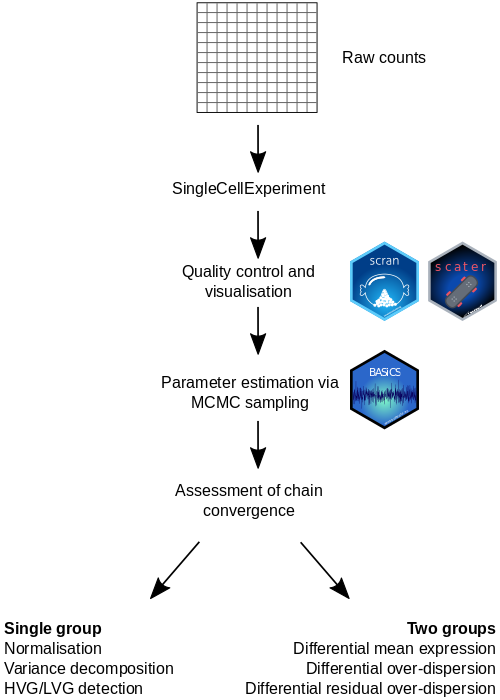
\includegraphics[width=2.5in,height=3.5in]{figure/Overview} 

}

\caption{Graphical overview for the scRNA-seq analysis workflow described in this manuscript. Starting from a matrix of expression counts, we use the scater and scran Bioconductor packages to perform QC and initial exploratory analyses. To robustly quantify transcriptional heterogeneity within seemingly homogeneous cell populations, we apply the BASiCS Bioconductor package and  illustrate how BASiCS can be used to analyse a single or multiple pre-specified groups of cells.}\label{fig:overview}
\end{figure}

\hypertarget{input-data}{%
\subsubsection{Input data}\label{input-data}}

\begin{Shaded}
\begin{Highlighting}[]
\KeywordTok{library}\NormalTok{(}\StringTok{"SingleCellExperiment"}\NormalTok{)}
\end{Highlighting}
\end{Shaded}

We use \emph{\href{https://bioconductor.org/packages/3.11/SingleCellExperiment}{SingleCellExperiment}} to convert an input
matrix of raw read-counts (molecule counts for UMI-based protocols) into a
\texttt{SingleCellExperiment} object that can also store its associated
metadata, such as gene- and cell-specific information.
Moreover, when available, the same object can also store read-counts for
spike-in molecules (see \texttt{?altExp}).
A major advantage of using a \texttt{SingleCellExperiment} object as the input for
scRNA-seq analyses is the interoperability across a large number of
Bioconductor packages \citep{Amezquita2019}.

\hypertarget{qc-and-exploratory-data-analysis}{%
\subsection{QC and exploratory data analysis}\label{qc-and-exploratory-data-analysis}}

\begin{Shaded}
\begin{Highlighting}[]
\KeywordTok{library}\NormalTok{(}\StringTok{"scater"}\NormalTok{)}
\KeywordTok{library}\NormalTok{(}\StringTok{"scran"}\NormalTok{)}
\end{Highlighting}
\end{Shaded}

An critical step in scRNA-seq analyses is QC, removing low quality samples that
may distort downstream analyses.
In this step, we use QC diagnostics to identify and remove samples that
correspond to broken cells, that are empty, or that contain multiple cells
\citep{Ilicic2016}. We also typically remove lowly expressed genes that represent
less reliable information.
The \href{https://osca.bioconductor.org/}{\emph{OSCA}} online book provides an extensive
overview on important aspects of how to perform QC of scRNA-seq data, including
exploratory analyses \citep{Amezquita2019}.

Here, we use the \emph{\href{https://bioconductor.org/packages/3.11/scater}{scater}} package \citep{McCarthy2017} to calculate
QC metrics for each cell (e.g.~total read-count) and gene (e.g.~percentage of
zeroes across all cells), respectively.
Moreover, we use the visualisation tools implemented in \emph{\href{https://bioconductor.org/packages/3.11/scater}{scater}} to
explore the input dataset and its associated QC diagnostic metrics.
For further data exploration we use the \emph{\href{https://bioconductor.org/packages/3.11/scran}{scran}} package \citep{Lun2016}.
\emph{\href{https://bioconductor.org/packages/3.11/scran}{scran}} can perform \emph{global scaling} normalisation, calculating
cell-specific scaling factors that capture global differences in read-counts
across cells (e.g.~due to sequencing depth and PCR amplification)
\citep{Lun2016pooling}.
Moreover, \emph{\href{https://bioconductor.org/packages/3.11/scran}{scran}} enables exploratory analyses of transcriptional
variability.
For example, it can be used to infer an overall trend between mean expression
and the squared coefficent of variation (CV\textsuperscript{2}) for each gene.
To derive variability estimates that are not confounded by this overall trend,
\emph{\href{https://bioconductor.org/packages/3.11/scran}{scran}} also defines gene-specific DM (distance to the mean)
estimates as the distance between CV\(^2\) and a rolling median along the range
of mean expression values \citep{Kolodziejczyk2015cell}.
DM estimates enable exploratory analyses of cell-to-cell heterogeneity, but a
measure of uncertainty is not readily available. As such, gene-specific
downstream inference (e.g.~differential variability testing) is precluded.

\hypertarget{basics---bayesian-analysis-of-single-cell-sequencing-data}{%
\subsection{BASiCS - Bayesian Analysis of Single Cell Sequencing data}\label{basics---bayesian-analysis-of-single-cell-sequencing-data}}

\begin{Shaded}
\begin{Highlighting}[]
\KeywordTok{library}\NormalTok{(}\StringTok{"BASiCS"}\NormalTok{)}
\end{Highlighting}
\end{Shaded}

The \emph{\href{https://bioconductor.org/packages/3.11/BASiCS}{BASiCS}} package uses a Bayesian hierarchical framework
that borrows information across all genes and cells to robustly quantify
transcriptional variability \citep{Vallejos2015BASiCS}.
Similar to the approach adopted in \emph{\href{https://bioconductor.org/packages/3.11/scran}{scran}}, \emph{\href{https://bioconductor.org/packages/3.11/BASiCS}{BASiCS}}
infers cell-specific global scaling normalisation parameters.
However, instead of inferring these as a pre-processing step,
\emph{\href{https://bioconductor.org/packages/3.11/BASiCS}{BASiCS}} uses an integrated approach wherein data normalisation
and downstream analyses are performed simultaneously, thereby propagating
statistical uncertainty.
To quantify technical noise, the original implementation of
\emph{\href{https://bioconductor.org/packages/3.11/BASiCS}{BASiCS}} uses information from extrinsic spike-in molecules as
control features, but the model has been extended to address situations wherein
spike-ins are not available \citep{Eling2018}.

\emph{\href{https://bioconductor.org/packages/3.11/BASiCS}{BASiCS}} summarises the expression pattern for each gene through
gene-specific \emph{mean} and \emph{over-dispersion} parameters.
Mean parameters \(\mu_i\) quantify the overall expression for each gene \(i\)
across the population of cells under study.
In contrast, \(\delta_i\) captures the excess of variability that is observed with
respect to what would be expected in a homogeneous cell population, after
taking into account technical noise.
This is used as a proxy to quantify transcriptional variability.
To account for the strong relationship that is typically observed
between gene-specific mean expression and over-dispersion estimates,
Eling \emph{et al.} \citep{Eling2018} recently introduced a joint prior specification for
these parameters.
This joint prior formulation has been observed to improve posterior inference
when the data is less informative (e.g.~small sample size, lowly expressed
genes), borroring information across all genes to infer an overall trend that
captures the relationship between mean and over-dispersion values.
The trend is subsequently used to derive gene-specific \emph{residual over-dispersion}
parameters \(\epsilon_i\) that are not confounded by mean expression.
Similar to DM values implemented in \emph{\href{https://bioconductor.org/packages/3.11/scran}{scran}}, these are defined as
deviations with respect to an overall regression trend .

Within a population of cells, \emph{\href{https://bioconductor.org/packages/3.11/BASiCS}{BASiCS}} decomposes the total
observed variability in expression measurements into technical and biological
components \citep{Vallejos2015}.
This enables the identification of \emph{highly variable genes} (HVGs) that capture
the major sources of heterogeneity within the analysed cells \citep{Brennecke2013}.
HVG detection is often used as feature selection, to identify the input
set of genes for subsequent analyses.
\emph{\href{https://bioconductor.org/packages/3.11/BASiCS}{BASiCS}} can also highlight \emph{lowly variable genes} (LVGs) that
exhibit stable expression across the population of cells.
These may relate to essential cellular functions and can assist the development
of new data normalisation or integration strategies \citep{Lin2019}.

\emph{\href{https://bioconductor.org/packages/3.11/BASiCS}{BASiCS}} also provides a probabilistic decision rule to
perform differential expression analyses between two (or more) pre-specified
groups of cells \citep{Vallejos2016, Eling2018}.
While several differential expression tools have been proposed for scRNA-seq
data (e.g. \citep{Kharchenko2014, Finak2015}), some evidence suggests that
these do not generally outperform popular bulk RNA-seq tools \citep{Soneson2018}.
Moreover, most of these methods are only designed to uncover changes in overall
expression, ignoring the more complex patterns that can arise at the single cell
level \citep{Lahnemann2020}.
Instead, \emph{\href{https://bioconductor.org/packages/3.11/BASiCS}{BASiCS}} embraces the high granularity of scRNA-seq data,
uncovering changes in cell-to-cell expression variability that are not
confounded by differences in technical noise or in overall expression.

\hypertarget{Tcells}{%
\section{\texorpdfstring{Case study: analysis of naive CD4\textsuperscript{+} T cells}{Case study: analysis of naive CD4+ T cells}}\label{Tcells}}

As a case study, we use scRNA-seq data generated for CD4\textsuperscript{+} T cells
using the C1 Single-Cell Auto Prep System (Fluidigm\textsuperscript{®}).
Martinez-Jimenez \emph{et al.} profiled naive (hereafter also referred to as
unstimulated) and activated (3 hours using \emph{in vitro} antibody stimulation)
CD4\textsuperscript{+} T cells from young and old animals across two mouse strains to study
changes in expression variability during ageing and upon immune activation
\citep{Martinez-jimenez2017}.
They extracted naive or effector memory CD4\textsuperscript{+} T cells from spleens of young or
old animals, obtaining purified populations using either magnetic-activated cell
sorting (MACS) or fluorescence activated cell sorting (FACS).
External ERCC spike-in RNA \citep{Rna2005} was added to aid the quantification of
technical variability across all cells and all experiments were performed in
replicates (hereafter also referred to as batches).

\hypertarget{downloading-the-data}{%
\subsection{Downloading the data}\label{downloading-the-data}}

The matrix with raw read counts can be obtained from ArrayExpress under the
accession number
\href{https://www.ebi.ac.uk/arrayexpress/experiments/E-MTAB-4888/}{E-MTAB-4888}.
In the matrix, column names contain library identifiers and row names
display gene Ensembl identifiers.

\begin{Shaded}
\begin{Highlighting}[]
\ControlFlowTok{if}\NormalTok{ (}\OperatorTok{!}\KeywordTok{file.exists}\NormalTok{(}\StringTok{"downloads/raw_data.txt"}\NormalTok{)) \{}
\NormalTok{  website <-}\StringTok{ "https://www.ebi.ac.uk/arrayexpress/files/E-MTAB-4888/"}
\NormalTok{  file <-}\StringTok{ "E-MTAB-4888.processed.1.zip"}
  \KeywordTok{download.file}\NormalTok{(}
    \KeywordTok{paste0}\NormalTok{(website, file),}
    \DataTypeTok{destfile =} \StringTok{"downloads/raw_data.txt.zip"}
\NormalTok{  )}
  \KeywordTok{unzip}\NormalTok{(}\StringTok{"downloads/raw_data.txt.zip"}\NormalTok{, }\DataTypeTok{exdir =} \StringTok{"downloads"}\NormalTok{)}
  \KeywordTok{file.remove}\NormalTok{(}\StringTok{"downloads/raw_data.txt.zip"}\NormalTok{)}
\NormalTok{\}}

\NormalTok{CD4_raw <-}\StringTok{ }\KeywordTok{read.table}\NormalTok{(}\StringTok{"downloads/raw_data.txt"}\NormalTok{, }\DataTypeTok{header =} \OtherTok{TRUE}\NormalTok{, }\DataTypeTok{sep =} \StringTok{"}\CharTok{\textbackslash{}t}\StringTok{"}\NormalTok{)}
\NormalTok{CD4_raw <-}\StringTok{ }\KeywordTok{as.matrix}\NormalTok{(CD4_raw)}
\end{Highlighting}
\end{Shaded}

The input matrix contains data for 1,513
cells and 31,181
genes (including 92 ERCC spike-ins).
Information about experimental conditions and other metadata is available
under the same accession number.

\begin{Shaded}
\begin{Highlighting}[]
\ControlFlowTok{if}\NormalTok{ (}\OperatorTok{!}\KeywordTok{file.exists}\NormalTok{(}\StringTok{"downloads/metadata_file.txt"}\NormalTok{)) \{}
\NormalTok{  website <-}\StringTok{ "https://www.ebi.ac.uk/arrayexpress/files/E-MTAB-4888"}
\NormalTok{  file <-}\StringTok{ "E-MTAB-4888.additional.1.zip"}
  \KeywordTok{download.file}\NormalTok{(}
    \KeywordTok{paste0}\NormalTok{(website, file),}
    \DataTypeTok{destfile =} \StringTok{"downloads/metadata.txt.zip"}
\NormalTok{  )}
  \KeywordTok{unzip}\NormalTok{(}\StringTok{"downloads/metadata.txt.zip"}\NormalTok{, }\DataTypeTok{exdir =} \StringTok{"downloads"}\NormalTok{)}
  \KeywordTok{file.remove}\NormalTok{(}\StringTok{"downloads/metadata.txt.zip"}\NormalTok{)}
\NormalTok{\}}

\NormalTok{CD4_metadata <-}\StringTok{ }\KeywordTok{read.table}\NormalTok{(}
  \StringTok{"downloads/metadata_file.txt"}\NormalTok{,}
  \DataTypeTok{header =} \OtherTok{TRUE}\NormalTok{,}
  \DataTypeTok{sep =} \StringTok{"}\CharTok{\textbackslash{}t}\StringTok{"}
\NormalTok{)}

\CommentTok{# Save sample identifiers as rownames}
\KeywordTok{rownames}\NormalTok{(CD4_metadata) <-}\StringTok{ }\NormalTok{CD4_metadata}\OperatorTok{$}\NormalTok{X}
\end{Highlighting}
\end{Shaded}

The columns in the metadata file contain library identifiers (\texttt{X}), strain
information (\texttt{Strain}; \emph{Mus musculus castaneus} or \emph{Mus musculus domesticus}),
the age of the animals (\texttt{Age}; young or old), stimulation state of the cells
(\texttt{Stimulus}; naive or activated), batch information (\texttt{Individuals}; associated
to different mice), and cell type information (\texttt{Celltype}; via FACS or MACS
purification).

Here, we convert the data and metadata described above into a
\texttt{SingleCellExperiment} object.
For this purpose, we first separate the input matrix of expression counts into
two matrices associated to intrinsic genes and external spike-ins, respectively.
Within the \texttt{SingleCellExperiment} object, the latter is stored separately
as an alternative experiment (see \texttt{?altExp}).

\begin{Shaded}
\begin{Highlighting}[]
\CommentTok{# Separate intrinsic from ERCC counts}
\NormalTok{bio_counts <-}\StringTok{ }\NormalTok{CD4_raw[}\OperatorTok{!}\KeywordTok{grepl}\NormalTok{(}\StringTok{"ERCC"}\NormalTok{, }\KeywordTok{rownames}\NormalTok{(CD4_raw)), ]}
\NormalTok{spike_counts <-}\StringTok{ }\NormalTok{CD4_raw[}\KeywordTok{grepl}\NormalTok{(}\StringTok{"ERCC"}\NormalTok{, }\KeywordTok{rownames}\NormalTok{(CD4_raw)), ]}
\CommentTok{# Generate the SingleCellExperiment object}
\NormalTok{sce_CD4_all <-}\StringTok{ }\KeywordTok{SingleCellExperiment}\NormalTok{(}
  \DataTypeTok{assays =} \KeywordTok{list}\NormalTok{(}\DataTypeTok{counts =} \KeywordTok{as.matrix}\NormalTok{(bio_counts)),}
  \DataTypeTok{colData =}\NormalTok{ CD4_metadata[}\KeywordTok{colnames}\NormalTok{(CD4_raw), ]}
\NormalTok{)}
\CommentTok{# Add read-counts for spike-ins as an alternative experiment}
\KeywordTok{altExp}\NormalTok{(sce_CD4_all, }\StringTok{"spike-ins"}\NormalTok{) <-}\StringTok{ }\KeywordTok{SummarizedExperiment}\NormalTok{(}
  \DataTypeTok{assays =} \KeywordTok{list}\NormalTok{(}\DataTypeTok{counts =}\NormalTok{ spike_counts)}
\NormalTok{)}
\end{Highlighting}
\end{Shaded}

Hereafter, our analysis focuses on naive and activated CD4\textsuperscript{+} T cells obtained
from young \emph{Mus musculus domesticus} animals, purified using MACS-based cell sorting.
Here, we extract these
146 samples.

\begin{Shaded}
\begin{Highlighting}[]
\NormalTok{ind_select <-}\StringTok{ }\NormalTok{sce_CD4_all}\OperatorTok{$}\NormalTok{Strain }\OperatorTok{==}\StringTok{ "Mus musculus domesticus"} \OperatorTok{&}
\StringTok{  }\NormalTok{sce_CD4_all}\OperatorTok{$}\NormalTok{Age }\OperatorTok{==}\StringTok{ "Young"} \OperatorTok{&}
\StringTok{  }\NormalTok{sce_CD4_all}\OperatorTok{$}\NormalTok{Celltype }\OperatorTok{==}\StringTok{ "MACS-purified Naive"}
\NormalTok{sce_naive_active <-}\StringTok{ }\NormalTok{sce_CD4_all[, ind_select]}
\NormalTok{sce_naive_active}
\end{Highlighting}
\end{Shaded}

\begin{verbatim}
## class: SingleCellExperiment 
## dim: 31089 146 
## metadata(0):
## assays(1): counts
## rownames(31089): ENSMUSG00000000001 ENSMUSG00000000003 ...
##   ENSMUSG00000106668 ENSMUSG00000106670
## rowData names(0):
## colnames(146): do6113 do6118 ... do6493 do6495
## colData names(6): X Strain ... Individuals Celltype
## reducedDimNames(0):
## altExpNames(1): spike-ins
\end{verbatim}

\hypertarget{qc-and-exploratory-data-analysis-1}{%
\subsection{QC and exploratory data analysis}\label{qc-and-exploratory-data-analysis-1}}

The data available at
\href{https://www.ebi.ac.uk/arrayexpress/experiments/E-MTAB-4888/}{E-MTAB-4888} have
been already filtered to remove poor quality samples.
The QC applied in \citep{Martinez-jimenez2017} removed cells with: (i) fewer
than 1,000,000 total reads, (ii) less than 20\% of reads mapped to
endogenous genes, (iii) less than 1,250 or more than 3,000 detected genes and
(iv) more than 10\% or fewer than 0.5\% of reads mapped to mitochondrial genes.
As an illustration, we visualise some of these metrics.
We also include another widely used QC diagnostic plot that compares the total
number (or fraction) of spike-in counts versus the total number (or fraction) of
endogeneous counts.
In such a plot, low quality samples are characterised by a high fraction of
spike-in counts and a low fraction of endogeneous counts
(see Figure \ref{fig:PerCellQC}).

\begin{Shaded}
\begin{Highlighting}[]
\CommentTok{# Calculate and plot per cell QC metrics}
\NormalTok{sce_naive_active <-}\StringTok{ }\KeywordTok{addPerCellQC}\NormalTok{(sce_naive_active, }\DataTypeTok{use_altexps =} \OtherTok{TRUE}\NormalTok{)}
\NormalTok{p_cellQC1 <-}\StringTok{ }\KeywordTok{plotColData}\NormalTok{(}
\NormalTok{  sce_naive_active, }
  \DataTypeTok{x =} \StringTok{"sum"}\NormalTok{, }
  \DataTypeTok{y =} \StringTok{"detected"}\NormalTok{) }\OperatorTok{+}
\StringTok{  }\KeywordTok{xlab}\NormalTok{(}\StringTok{"Total engogenous reads per cell"}\NormalTok{) }\OperatorTok{+}
\StringTok{  }\KeywordTok{ylab}\NormalTok{(}\StringTok{"Number of detected genes per cell"}\NormalTok{) }\OperatorTok{+}
\StringTok{  }\KeywordTok{theme}\NormalTok{(}\DataTypeTok{axis.text.x =} \KeywordTok{element_text}\NormalTok{(}\DataTypeTok{hjust =} \DecValTok{1}\NormalTok{, }\DataTypeTok{angle =} \DecValTok{45}\NormalTok{))}
\NormalTok{p_cellQC2 <-}\StringTok{ }\KeywordTok{plotColData}\NormalTok{(}
\NormalTok{  sce_naive_active, }
  \DataTypeTok{x =} \StringTok{"sum"}\NormalTok{, }
  \DataTypeTok{y =} \StringTok{"altexps_spike-ins_sum"}\NormalTok{) }\OperatorTok{+}
\StringTok{  }\KeywordTok{xlab}\NormalTok{(}\StringTok{"Total engogenous reads per cell"}\NormalTok{) }\OperatorTok{+}
\StringTok{  }\KeywordTok{ylab}\NormalTok{(}\StringTok{"Total spike-in reads per cell"}\NormalTok{) }\OperatorTok{+}
\StringTok{  }\KeywordTok{theme}\NormalTok{(}\DataTypeTok{axis.text.x =} \KeywordTok{element_text}\NormalTok{(}\DataTypeTok{hjust =} \DecValTok{1}\NormalTok{, }\DataTypeTok{angle =} \DecValTok{45}\NormalTok{))}
\KeywordTok{multiplot}\NormalTok{(p_cellQC1, p_cellQC2, }\DataTypeTok{cols =} \DecValTok{2}\NormalTok{)}
\end{Highlighting}
\end{Shaded}

\begin{figure}

{\centering \includegraphics{figure/PerCellQC-1} 

}

\caption{Cell-level QC metrics. The total number of endogenous read-counts (excludes non-mapped and intronic reads) is plotted against the total number of detected genes (left) and the total number of spike-in read-counts (right).}\label{fig:PerCellQC}
\end{figure}

We can also visualise these metrics with respect to cell-level metadata, such
as the experimental conditions (active vs unstimulated) and the different mice
that cells were collected from
(see Figure \ref{fig:experimental-condition-batch}).

\begin{Shaded}
\begin{Highlighting}[]
\NormalTok{p_stimulus <-}\StringTok{ }\KeywordTok{plotColData}\NormalTok{(}
\NormalTok{    sce_naive_active,}
    \DataTypeTok{x =} \StringTok{"sum"}\NormalTok{,}
    \DataTypeTok{y =} \StringTok{"detected"}\NormalTok{, }
    \DataTypeTok{colour_by =} \StringTok{"Stimulus"}\NormalTok{) }\OperatorTok{+}
\StringTok{  }\KeywordTok{xlab}\NormalTok{(}\StringTok{"Total engogenous reads per cell"}\NormalTok{) }\OperatorTok{+}
\StringTok{  }\KeywordTok{ylab}\NormalTok{(}\StringTok{"Number of detected genes per cell"}\NormalTok{) }\OperatorTok{+}
\StringTok{  }\KeywordTok{theme}\NormalTok{(}
    \DataTypeTok{legend.position =} \StringTok{"bottom"}\NormalTok{,}
    \DataTypeTok{axis.text.x =} \KeywordTok{element_text}\NormalTok{(}\DataTypeTok{angle =} \DecValTok{45}\NormalTok{, }\DataTypeTok{hjust =} \DecValTok{1}\NormalTok{))}
\NormalTok{p_batch <-}\StringTok{ }\KeywordTok{plotColData}\NormalTok{(}
\NormalTok{    sce_naive_active,}
    \DataTypeTok{x =} \StringTok{"sum"}\NormalTok{,}
    \DataTypeTok{y =} \StringTok{"detected"}\NormalTok{, }
    \DataTypeTok{colour_by =} \StringTok{"Individuals"}\NormalTok{) }\OperatorTok{+}
\StringTok{  }\KeywordTok{xlab}\NormalTok{(}\StringTok{"Total engogenous reads per cell"}\NormalTok{) }\OperatorTok{+}
\StringTok{  }\KeywordTok{ylab}\NormalTok{(}\StringTok{"Number of detected genes per cell"}\NormalTok{) }\OperatorTok{+}
\StringTok{  }\KeywordTok{theme}\NormalTok{(}
    \DataTypeTok{legend.position =} \StringTok{"bottom"}\NormalTok{,}
    \DataTypeTok{axis.text.x =} \KeywordTok{element_text}\NormalTok{(}\DataTypeTok{angle =} \DecValTok{45}\NormalTok{, }\DataTypeTok{hjust =} \DecValTok{1}\NormalTok{))}
\KeywordTok{multiplot}\NormalTok{(p_stimulus, p_batch, }\DataTypeTok{cols =} \DecValTok{2}\NormalTok{)}
\end{Highlighting}
\end{Shaded}

\begin{figure}

{\centering \includegraphics{figure/experimental-condition-batch-1} 

}

\caption{Cell-level QC metrics according to cell-level metadata. The total number of endogenous reads (excludes non-mapped and intronic reads) is plotted against the total number of detected genes. Colour indicates the experimental condition (left) and animal of origin (right) for each cell.}\label{fig:experimental-condition-batch}
\end{figure}

To further explore the underlying structure of the data, we compute global
scaling normalisation factors using \emph{\href{https://bioconductor.org/packages/3.11/scran}{scran}} and perform a
principal component analysis (PCA) of log-transformed normalised expression
counts using \emph{\href{https://bioconductor.org/packages/3.11/scater}{scater}}.
As seen in Figure \ref{fig:pca-visualisation-stimulus-batch}, this analysis
suggests the absence of strong batch effects.
It should be noted that \emph{\href{https://bioconductor.org/packages/3.11/scran}{scran}} normalisation
is not strictly necessary in the \emph{\href{https://bioconductor.org/packages/3.11/BASiCS}{BASiCS}} workflow and we only
use it here as part of the exploratory data analysis.
Moreover, count-based models for dimensionality reduction (e.g. \citep{Townes2019, Lopez2018}) could be used as an alternative to PCA,
removing the need for log normalisation .

\begin{Shaded}
\begin{Highlighting}[]
\CommentTok{# Global scaling normalisation + log tranformation + PCA}
\NormalTok{sce_naive_active <-}\StringTok{ }\KeywordTok{computeSumFactors}\NormalTok{(sce_naive_active)}
\NormalTok{sce_naive_active <-}\StringTok{ }\KeywordTok{logNormCounts}\NormalTok{(sce_naive_active)}
\NormalTok{sce_naive_active <-}\StringTok{ }\KeywordTok{runPCA}\NormalTok{(sce_naive_active)}
\NormalTok{p_stimulus <-}\StringTok{ }\KeywordTok{plotPCA}\NormalTok{(sce_naive_active, }\DataTypeTok{colour_by =} \StringTok{"Stimulus"}\NormalTok{) }\OperatorTok{+}
\StringTok{  }\KeywordTok{theme}\NormalTok{(}\DataTypeTok{legend.position =} \StringTok{"bottom"}\NormalTok{)}
\NormalTok{p_batch <-}\StringTok{ }\KeywordTok{plotPCA}\NormalTok{(sce_naive_active, }\DataTypeTok{colour_by =} \StringTok{"Individuals"}\NormalTok{) }\OperatorTok{+}
\StringTok{  }\KeywordTok{theme}\NormalTok{(}\DataTypeTok{legend.position =} \StringTok{"bottom"}\NormalTok{)}
\KeywordTok{multiplot}\NormalTok{(p_stimulus, p_batch, }\DataTypeTok{cols =} \DecValTok{2}\NormalTok{)}
\end{Highlighting}
\end{Shaded}

\begin{figure}

{\centering \includegraphics{figure/pca-visualisation-stimulus-batch-1} 

}

\caption{First two principal components of log-transformed expression counts after scran normalisation. Colour indicates the experimental condition (left) and animal of origin (right) for each cell.}\label{fig:pca-visualisation-stimulus-batch}
\end{figure}

In addition to cell-specific QC, we also recommend the use of a gene filtering
step prior to the use of \emph{\href{https://bioconductor.org/packages/3.11/BASiCS}{BASiCS}}.
The purpose of this filter is to remove lowly expressed genes that were largely
undetected through sequencing, making reliable variability estimates difficult
to obtain.
Here, we remove all genes that are not detected in at least 5 cells across both
experimental conditions or that have an average read count below 1.
These thresholds can vary across datasets and should be informed by
gene-specific QC metrics such as those shown in
Figure \ref{fig:gene-selection}.

\begin{Shaded}
\begin{Highlighting}[]
\CommentTok{# Calculate per gene QC metrics}
\NormalTok{sce_naive_active <-}\StringTok{ }\KeywordTok{addPerFeatureQC}\NormalTok{(sce_naive_active, }\DataTypeTok{exprs_values =} \StringTok{"counts"}\NormalTok{)}
\CommentTok{# Remove genes with zero total counts across all cells}
\NormalTok{sce_naive_active <-}\StringTok{ }\NormalTok{sce_naive_active[}\KeywordTok{rowData}\NormalTok{(sce_naive_active)}\OperatorTok{$}\NormalTok{detected }\OperatorTok{!=}\StringTok{ }\DecValTok{0}\NormalTok{, ]}
\CommentTok{# Transform 'detected' metadata into number of cells }
\KeywordTok{rowData}\NormalTok{(sce_naive_active)}\OperatorTok{$}\NormalTok{detected_cells <-}\StringTok{ }
\StringTok{  }\KeywordTok{rowData}\NormalTok{(sce_naive_active)}\OperatorTok{$}\NormalTok{detected }\OperatorTok{*}\StringTok{ }\KeywordTok{ncol}\NormalTok{(sce_naive_active) }\OperatorTok{/}\StringTok{ }\DecValTok{100}
\CommentTok{# Define inclusion criteria for genes}
\KeywordTok{rowData}\NormalTok{(sce_naive_active)}\OperatorTok{$}\NormalTok{include_gene <-}\StringTok{ }\KeywordTok{rowData}\NormalTok{(sce_naive_active)}\OperatorTok{$}\NormalTok{mean }\OperatorTok{>=}\StringTok{ }\DecValTok{1} \OperatorTok{&}
\StringTok{  }\KeywordTok{rowData}\NormalTok{(sce_naive_active)}\OperatorTok{$}\NormalTok{detected_cells }\OperatorTok{>=}\StringTok{ }\DecValTok{5}
\KeywordTok{plotRowData}\NormalTok{(}
\NormalTok{    sce_naive_active,}
    \DataTypeTok{x =} \StringTok{"detected_cells"}\NormalTok{,}
    \DataTypeTok{y =} \StringTok{"mean"}\NormalTok{,}
    \DataTypeTok{colour_by =} \StringTok{"include_gene"}\NormalTok{) }\OperatorTok{+}
\StringTok{  }\KeywordTok{xlab}\NormalTok{(}\StringTok{"Total engogenous reads per cell"}\NormalTok{) }\OperatorTok{+}
\StringTok{  }\KeywordTok{ylab}\NormalTok{(}\StringTok{"Number of detected genes per cell"}\NormalTok{) }\OperatorTok{+}
\StringTok{  }\KeywordTok{scale_x_log10}\NormalTok{() }\OperatorTok{+}
\StringTok{  }\KeywordTok{scale_y_log10}\NormalTok{() }\OperatorTok{+}
\StringTok{  }\KeywordTok{theme}\NormalTok{(}
    \DataTypeTok{legend.position =} \StringTok{"bottom"}\NormalTok{,}
    \DataTypeTok{axis.text.x =} \KeywordTok{element_text}\NormalTok{(}\DataTypeTok{angle =} \DecValTok{45}\NormalTok{, }\DataTypeTok{hjust =} \DecValTok{1}\NormalTok{)) }\OperatorTok{+}
\KeywordTok{geom_vline}\NormalTok{(}\DataTypeTok{xintercept =} \DecValTok{5}\NormalTok{, }\DataTypeTok{linetype =} \StringTok{"dashed"}\NormalTok{, }\DataTypeTok{col =} \StringTok{"grey60"}\NormalTok{) }\OperatorTok{+}
\KeywordTok{geom_hline}\NormalTok{(}\DataTypeTok{yintercept =} \DecValTok{1}\NormalTok{, }\DataTypeTok{linetype =} \StringTok{"dashed"}\NormalTok{, }\DataTypeTok{col =} \StringTok{"grey60"}\NormalTok{)}
\end{Highlighting}
\end{Shaded}

\begin{figure}

{\centering \includegraphics{figure/gene-selection-1} 

}

\caption{Average read-count for each gene is plotted against the number of cells in which that gene was detected. Dashed grey lines are shown at the thresholds below which genes are removed.}\label{fig:gene-selection}
\end{figure}

\begin{Shaded}
\begin{Highlighting}[]
\CommentTok{# Apply gene filter}
\NormalTok{sce_naive_active <-}\StringTok{ }\NormalTok{sce_naive_active[}\KeywordTok{rowData}\NormalTok{(sce_naive_active)}\OperatorTok{$}\NormalTok{include_gene, ]}
\end{Highlighting}
\end{Shaded}

Subsequently, we also require users to remove spike-in molecules that were not
captured through sequencing. We will do this separately for naive and active
cells separately.

\begin{Shaded}
\begin{Highlighting}[]
\NormalTok{ind_active <-}\StringTok{ }\NormalTok{sce_naive_active}\OperatorTok{$}\NormalTok{Stimulus }\OperatorTok{==}\StringTok{ "Active"}
\NormalTok{ind_naive <-}\StringTok{ }\NormalTok{sce_naive_active}\OperatorTok{$}\NormalTok{Stimulus }\OperatorTok{==}\StringTok{ "Unstimulated"}
\NormalTok{spikes <-}\StringTok{ }\KeywordTok{assay}\NormalTok{(}\KeywordTok{altExp}\NormalTok{(sce_naive_active))}
\NormalTok{detected_spikes_active <-}\StringTok{ }\KeywordTok{rowSums}\NormalTok{(spikes[, ind_active] }\OperatorTok{>}\StringTok{ }\DecValTok{0}\NormalTok{) }\OperatorTok{>}\StringTok{ }\DecValTok{0}
\NormalTok{detected_spikes_naive <-}\StringTok{ }\KeywordTok{rowSums}\NormalTok{(spikes[, ind_naive] }\OperatorTok{>}\StringTok{ }\DecValTok{0}\NormalTok{) }\OperatorTok{>}\StringTok{ }\DecValTok{0}
\NormalTok{detected_spikes <-}\StringTok{ }\NormalTok{detected_spikes_naive }\OperatorTok{&}\StringTok{ }\NormalTok{detected_spikes_active}
\KeywordTok{altExp}\NormalTok{(sce_naive_active) <-}\StringTok{ }\KeywordTok{altExp}\NormalTok{(sce_naive_active)[detected_spikes, ]}
\end{Highlighting}
\end{Shaded}

The final dataset used in subsequent analyses contains
146 cells, 8953 genes and
49 spike-ins.

\hypertarget{input-data-for-basics}{%
\subsection{Input data for BASiCS}\label{input-data-for-basics}}

Here, we apply the \emph{\href{https://bioconductor.org/packages/3.11/BASiCS}{BASiCS}} model separately to cells from each
experimental condition (93
naive and 53 activated cells).
We create separate \texttt{SingleCellExperiment} objects for each group of cells.

\begin{Shaded}
\begin{Highlighting}[]
\NormalTok{sce_naive <-}\StringTok{ }\NormalTok{sce_naive_active[, ind_naive]}
\NormalTok{sce_active <-}\StringTok{ }\NormalTok{sce_naive_active[, ind_active]}
\end{Highlighting}
\end{Shaded}

\emph{\href{https://bioconductor.org/packages/3.11/BASiCS}{BASiCS}} requires the user to update these objects with additional
information, using a specific format.
Firstly, if multiple batches of sequenced cells are available (e.g.~multiple
donors that cells were extracted from, or multiple sequencing batches from the
same experimental condition), this information must be included under the
\texttt{BatchInfo} label as part of the cell-level metadata.

\begin{Shaded}
\begin{Highlighting}[]
\KeywordTok{colData}\NormalTok{(sce_naive)}\OperatorTok{$}\NormalTok{BatchInfo <-}\StringTok{ }\KeywordTok{colData}\NormalTok{(sce_naive)}\OperatorTok{$}\NormalTok{Individuals}
\KeywordTok{colData}\NormalTok{(sce_active)}\OperatorTok{$}\NormalTok{BatchInfo <-}\StringTok{ }\KeywordTok{colData}\NormalTok{(sce_active)}\OperatorTok{$}\NormalTok{Individuals}
\end{Highlighting}
\end{Shaded}

If spike-ins will be used to aid data normalisation and technical noise
quantification, \emph{\href{https://bioconductor.org/packages/3.11/BASiCS}{BASiCS}} also requires the number of spike-in
molecules that were added to each well.
For each spike-in gene \(i\), this corresponds to:

\[ \mu_{i} = C_i \times 10^{-18} \times (6.022 \times 10^{23}) 
\times V \times D \hspace{0.5cm} \mbox{where,} \]

\begin{itemize}
\item
  \(C_i\) is the concentration for the spike-in \(i\) (measured in \(aM\mu{}l^{-1}\)),
\item
  \(V\) is the volume added into each well (measure in \(nl\)) and
\item
  \(D\) is a dilution factor.
\end{itemize}

The remaining factors in the equation above are unit conversion constants
(e.g.~from moles to molecules).
For the CD4\textsuperscript{+} T cell data, the authors added a 1:50,000 dilution of the ERCC
spike-in mix 1 and a volume of \(9nl\) was added into each well (see \url{https://www.fluidigm.com/faq/ifc-9}).
Finally, input concentrations \(C_i\) can be downloaded from
\href{https://assets.thermofisher.com/TFS-Assets/LSG/manuals/cms_095046.txt}{https://assets.thermofisher.com/TFS-Assets/LSG/manuals}.

\begin{Shaded}
\begin{Highlighting}[]
\ControlFlowTok{if}\NormalTok{ (}\OperatorTok{!}\KeywordTok{file.exists}\NormalTok{(}\StringTok{"downloads/spike_info.txt"}\NormalTok{)) \{}
\NormalTok{  website <-}\StringTok{ "https://assets.thermofisher.com/TFS-Assets/LSG/manuals"}
\NormalTok{  file <-}\StringTok{ "cms_095046.txt"}
  \KeywordTok{download.file}\NormalTok{(}
    \KeywordTok{paste0}\NormalTok{(website, file),}
    \DataTypeTok{destfile =} \StringTok{"downloads/spike_info.txt"}
\NormalTok{  )  }
\NormalTok{\}}

\NormalTok{ERCC_conc <-}\StringTok{ }\KeywordTok{read.table}\NormalTok{(}\StringTok{"downloads/spike_info.txt"}\NormalTok{, }\DataTypeTok{sep =} \StringTok{"}\CharTok{\textbackslash{}t}\StringTok{"}\NormalTok{, }\DataTypeTok{header =} \OtherTok{TRUE}\NormalTok{)}
\end{Highlighting}
\end{Shaded}

Based on this information, the calculation above proceeds as follows

\begin{Shaded}
\begin{Highlighting}[]
\CommentTok{# Moles per micro litre}
\NormalTok{ERCC_mmul <-}\StringTok{ }\NormalTok{ERCC_conc}\OperatorTok{$}\NormalTok{concentration.in.Mix.}\DecValTok{1}\NormalTok{..attomoles.ul. }\OperatorTok{*}\StringTok{ }\NormalTok{(}\DecValTok{10}\OperatorTok{^}\NormalTok{(}\OperatorTok{-}\DecValTok{18}\NormalTok{))}
\CommentTok{# Molecule count per micro litre (1 mole comprises 6.02214076 x 10^\{23\} molecules)}
\NormalTok{ERCC_countmul <-}\StringTok{ }\NormalTok{ERCC_mmul }\OperatorTok{*}\StringTok{ }\NormalTok{(}\FloatTok{6.02214076} \OperatorTok{*}\StringTok{ }\NormalTok{(}\DecValTok{10}\OperatorTok{^}\DecValTok{23}\NormalTok{))}
\CommentTok{# Application of the dilution factor (1:50,000)}
\NormalTok{ERCC_count <-}\StringTok{ }\NormalTok{ERCC_countmul }\OperatorTok{/}\StringTok{ }\DecValTok{50000}
\CommentTok{# Multiplying by the volume added into each well}
\NormalTok{ERCC_count_final <-}\StringTok{ }\NormalTok{ERCC_count }\OperatorTok{*}\StringTok{ }\FloatTok{0.009}
\end{Highlighting}
\end{Shaded}

To update the \texttt{sce\_naive} and \texttt{sce\_active} objects, the user must create a
\texttt{data.frame} whose first column contains the labels associated to
the spike-in molecule (e.g.~ERCC-00130) and whose second column contains the
input number of molecules calculated above.
We add this information as metadata for \texttt{altExp(sce\_naive)} and
\texttt{altExp(sce\_active)}, respectively.

\begin{Shaded}
\begin{Highlighting}[]
\NormalTok{SpikeInput <-}\StringTok{ }\KeywordTok{data.frame}\NormalTok{(}
  \DataTypeTok{Names =}\NormalTok{ ERCC_conc}\OperatorTok{$}\NormalTok{ERCC.ID,}
  \DataTypeTok{count =}\NormalTok{ ERCC_count_final}
\NormalTok{)}
\CommentTok{# Exclude spike-ins not included in the input SingleCellExperiment objects}
\CommentTok{# and ensure the order of the rows is identical}
\NormalTok{SpikeInput <-}\StringTok{ }\NormalTok{SpikeInput[}\KeywordTok{match}\NormalTok{(}\KeywordTok{rownames}\NormalTok{(}\KeywordTok{altExp}\NormalTok{(sce_naive)), SpikeInput}\OperatorTok{$}\NormalTok{Names), ]}

\KeywordTok{metadata}\NormalTok{(sce_naive)}\OperatorTok{$}\NormalTok{SpikeInput <-}\StringTok{ }\NormalTok{SpikeInput}
\KeywordTok{metadata}\NormalTok{(sce_active)}\OperatorTok{$}\NormalTok{SpikeInput <-}\StringTok{ }\NormalTok{SpikeInput}
\end{Highlighting}
\end{Shaded}

\hypertarget{parameter-estimation-using-basics}{%
\subsection{Parameter estimation using BASiCS}\label{parameter-estimation-using-basics}}

Parameter estimation is implemented in the \texttt{BASiCS\_MCMC} function using an
adaptive Metropolis within Gibbs algorithm \citep{Roberts2009}.
The primary inputs for \texttt{BASiCS\_MCMC} correspond to:

\begin{itemize}
\item
  \texttt{Data}: a \texttt{SingleCellExperiment} object created as described in the
  previous sections.
\item
  \texttt{N}: the total number of MCMC iterations.
\item
  \texttt{Thin}: thining period for output storage
  (only the \texttt{Thin}-th MCMC draw is stored).
\item
  \texttt{Burn}: the initial number of MCMC iterations to be discarded.
\item
  \texttt{Regression}: if \texttt{TRUE} a join prior is assigned to \(\mu_i\) and \(\delta_i\)
  \citep{Eling2018}, and residual over-dispersion values \(\epsilon_i\) are inferred.
  Alternatively, independent log-normal priors are assigned to \(\mu_i\) and
  \(\delta_i\) \citep{Vallejos2016}.
\item
  \texttt{WithSpikes}: if \texttt{TRUE} information from spike-in molecules is used to aid
  data normalisation and to quantify technical noise.
\end{itemize}

As a default, we recommend to use \texttt{Regression\ =\ TRUE} as we have observed that
the joint prior introduced by Eling \emph{et al.} leads to improved inference for
small sample sizes and lowly expressed genes.
Moreover, the joint prior formulation enables users to obtain a measure of
transcriptional variability that is not confounded by mean expression.
Additional optional parameters can be used to store the generated output
(\texttt{StoreChains}, \texttt{StoreDir}, \texttt{RunName}) and to monitor the progress of the
algorithm (\texttt{PrintProgress}).

Here, we run the MCMC sampler separately for naive and activated cells.
We use 40,000 iterations, discarding the initial 20,000 iterations.
We recommend this setting as a default choice, as we have observed it to
ensure good convergence for the algorithm across multiple datasets.
However, for large datasets and less sparse datasets, a lower number of
iterations may be sufficient.
Practical guidance about the diagnostics criteria required to assess the
performance of the MCMC algorithn is provided in the next section.

\begin{Shaded}
\begin{Highlighting}[]
\NormalTok{chain_naive <-}\StringTok{ }\KeywordTok{BASiCS_MCMC}\NormalTok{(}
  \DataTypeTok{Data =}\NormalTok{ sce_naive,}
  \DataTypeTok{N =} \DecValTok{40000}\NormalTok{,}
  \DataTypeTok{Thin =} \DecValTok{20}\NormalTok{,}
  \DataTypeTok{Burn =} \DecValTok{20000}\NormalTok{,}
  \DataTypeTok{Regression =} \OtherTok{TRUE}\NormalTok{,}
  \DataTypeTok{WithSpikes =} \OtherTok{TRUE}\NormalTok{,}
  \DataTypeTok{StoreChains =} \OtherTok{TRUE}\NormalTok{,}
  \DataTypeTok{StoreDir =} \StringTok{"rds/"}\NormalTok{,}
  \DataTypeTok{RunName =} \StringTok{"naive"}
\NormalTok{)}

\NormalTok{chain_active <-}\StringTok{ }\KeywordTok{BASiCS_MCMC}\NormalTok{(}
  \DataTypeTok{Data =}\NormalTok{ sce_active,}
  \DataTypeTok{N =} \DecValTok{40000}\NormalTok{,}
  \DataTypeTok{Thin =} \DecValTok{20}\NormalTok{,}
  \DataTypeTok{Burn =} \DecValTok{20000}\NormalTok{,}
  \DataTypeTok{Regression =} \OtherTok{TRUE}\NormalTok{,}
  \DataTypeTok{WithSpikes =} \OtherTok{TRUE}\NormalTok{,}
  \DataTypeTok{StoreChains =} \OtherTok{TRUE}\NormalTok{,}
  \DataTypeTok{StoreDir =} \StringTok{"rds/"}\NormalTok{,}
  \DataTypeTok{RunName =} \StringTok{"active"}
\NormalTok{)}
\end{Highlighting}
\end{Shaded}

This first of these samplers takes 127 minutes to complete on a 3.4 GHz Intel
Core i7 4770k procesor with 16GB RAM, while the second takes 75 minutes.
For convenience, these can be obtained online at
\url{https://git.ecdf.ed.ac.uk/vallejosgroup/basicsworkflow2020}.

\begin{Shaded}
\begin{Highlighting}[]
\ControlFlowTok{if}\NormalTok{ (}\OperatorTok{!}\KeywordTok{file.exists}\NormalTok{(}\StringTok{"rds/chain_naive.Rds"}\NormalTok{)) \{}
\NormalTok{  website <-}\StringTok{ "https://git.ecdf.ed.ac.uk/vallejosgroup/basicsworkflow2020/raw/master/"}
\NormalTok{  file <-}\StringTok{ "chain_naive.Rds"}
  \KeywordTok{download.file}\NormalTok{(}
    \KeywordTok{paste0}\NormalTok{(website, file),}
    \DataTypeTok{destfile =} \StringTok{"rds/chain_naive.Rds"}
\NormalTok{  )  }
\NormalTok{\}}
\ControlFlowTok{if}\NormalTok{ (}\OperatorTok{!}\KeywordTok{file.exists}\NormalTok{(}\StringTok{"rds/chain_active.Rds"}\NormalTok{)) \{}
\NormalTok{  website <-}\StringTok{ "https://git.ecdf.ed.ac.uk/vallejosgroup/basicsworkflow2020/raw/master/"}
\NormalTok{  file <-}\StringTok{ "chain_active.Rds"}
  \KeywordTok{download.file}\NormalTok{(}
    \KeywordTok{paste0}\NormalTok{(website, file),}
    \DataTypeTok{destfile =} \StringTok{"rds/chain_active.Rds"}
\NormalTok{  )  }
\NormalTok{\}}
\NormalTok{chain_naive <-}\StringTok{ }\KeywordTok{readRDS}\NormalTok{(}\StringTok{"rds/chain_naive.Rds"}\NormalTok{)}
\NormalTok{chain_active <-}\StringTok{ }\KeywordTok{readRDS}\NormalTok{(}\StringTok{"rds/chain_active.Rds"}\NormalTok{)}
\end{Highlighting}
\end{Shaded}

The output from \texttt{BASiCS\_MCMC} is a \texttt{BASiCS\_Chain} object that contains the
draws associated to all model parameters (as \texttt{N} = 40,000, \texttt{Thin} = 20 and
\texttt{Burn} = 20,000, the object contains 1,000 draws for each parameter).
These can be accessed using the \texttt{displayChainBASiCS} function.
For example, the following code displays the first 2 draws for mean
expression parameters \(\mu_i\) associated to the first 3 genes.

\begin{Shaded}
\begin{Highlighting}[]
\KeywordTok{displayChainBASiCS}\NormalTok{(chain_naive, }\DataTypeTok{Param =} \StringTok{"mu"}\NormalTok{)[}\DecValTok{1}\OperatorTok{:}\DecValTok{2}\NormalTok{, }\DecValTok{1}\OperatorTok{:}\DecValTok{3}\NormalTok{]}
\end{Highlighting}
\end{Shaded}

\begin{verbatim}
##      ENSMUSG00000000001 ENSMUSG00000000056 ENSMUSG00000000085
## [1,]           11.90910           1.854180          0.9695263
## [2,]           14.97279           1.625154          0.8400265
\end{verbatim}

\hypertarget{mcmc-diagnostics}{%
\subsection{MCMC diagnostics}\label{mcmc-diagnostics}}

Before interpreting the parameter estimates obtained by \emph{\href{https://bioconductor.org/packages/3.11/BASiCS}{BASiCS}},
it is critical to assess the convergence of the MCMC algorithm, i.e.~whether
the MCMC reached its stationary distribution.
If convergence has been achieved, each parameter should not (on average) evolve
significantly over time, and draws are expected to be stochastic fluctuations
around a horizontal trend.
Generally, it is not possible to prove convergence but multiple graphical and
quantitative convergence diagnostics have been proposed to assess the lack
of convergence (e.g. \citep{CowlesCarlin1996, BrooksGelman1998}).
Some advocate the use of multiple MCMC chains using different starting values in
order to ensure that the algorithm consistently converges to the same
distribution.
For \emph{\href{https://bioconductor.org/packages/3.11/BASiCS}{BASiCS}}, we have observed that using informed starting values
(e.g.~based on \emph{\href{https://bioconductor.org/packages/3.11/scran}{scran}} normalisation) and a sufficiently large
value for \texttt{N} and \texttt{Burn} generally leads to consistent across multiple MCMC runs.
Hence, the focus of this section is to evaluate quantitative measures of
convergence (e.g. \citep{Geweke1995}) based on a single MCMC chain.

Traceplots can be used to visually assess the history of posterior draws
generated by the algorithm for a specific parameter (e.g.~Figure
\ref{fig:convergence-naive}).
As mentioned above, significan departures from a horizontal trend suggest a
lack of convergence.
As illustrated in Figure \ref{fig:convergence-naive}, histograms can also be
used to display the marginal distribution for each parameter.
Users should expect these to follow a unimodal distribution.
Failure to satisfy these graphical diagnostics suggest that \texttt{N} and \texttt{Burn} must
be increased.
Alternatively, more stringent quality control could be applied to the input
data, as genes with very low counts often suffer from slow convergence and poor sampling efficiency.

\begin{Shaded}
\begin{Highlighting}[]
\KeywordTok{plot}\NormalTok{(chain_naive, }\DataTypeTok{Param =} \StringTok{"mu"}\NormalTok{, }\DataTypeTok{Gene =} \DecValTok{1}\NormalTok{)}
\end{Highlighting}
\end{Shaded}

\begin{figure}

{\centering \includegraphics{figure/convergence-naive-1} 

}

\caption{Trace plot, marginal histogram, and autocorrelation function for a gene in naive cells following MCMC sampling. Trace plots should explore the posterior well, without getting stuck in one location or drifting over time towards a region of higher density. High autocorrelation indicates that the number of effective independent samples is low. It is good practice to perform these visualisation for many different parameters; here we only show one.}\label{fig:convergence-naive}
\end{figure}

As \emph{\href{https://bioconductor.org/packages/3.11/BASiCS}{BASiCS}} infers thousands of parameters, it is
impractical to assess these graphical diagnostics for each parameter.
Thus, it is helpful to use numerical diagnostics that can be applied to multiple
parameters simultaneously to judge whether the algorithm has failed to converge.
Here, we focus on the diagnostic criterion proposed by Geweke \citep{Geweke1995}
which compares the average draws obtained during the initial (10\% after burn
in, by default) and the final part of the chain (50\% by default).
Large absolute Z-scores suggest that the algorithm has not converged.
For the naive and activatived CD4\textsuperscript{+} T datasets most Z-scores associated to mean
expression parameters \(\mu_i\) were small in aboslute value (see Figure \ref{fig:geweke-diag}).

\begin{Shaded}
\begin{Highlighting}[]
\KeywordTok{library}\NormalTok{(}\StringTok{"coda"}\NormalTok{)}
\KeywordTok{library}\NormalTok{(}\StringTok{"ggplot2"}\NormalTok{)}
\KeywordTok{library}\NormalTok{(}\StringTok{"viridis"}\NormalTok{)}

\CommentTok{# Calculate and plot Geweke Z scores }
\NormalTok{gew_mu_naive <-}\StringTok{ }\KeywordTok{geweke.diag}\NormalTok{(}\KeywordTok{mcmc}\NormalTok{(}\KeywordTok{displayChainBASiCS}\NormalTok{(chain_naive, }\DataTypeTok{Param =} \StringTok{"mu"}\NormalTok{)))}\OperatorTok{$}\NormalTok{z}
\NormalTok{gew_mu_active <-}\StringTok{ }\KeywordTok{geweke.diag}\NormalTok{(}\KeywordTok{mcmc}\NormalTok{(}\KeywordTok{displayChainBASiCS}\NormalTok{(chain_active, }\DataTypeTok{Param =} \StringTok{"mu"}\NormalTok{)))}\OperatorTok{$}\NormalTok{z}

\NormalTok{myplot_params <-}\StringTok{ }\KeywordTok{list}\NormalTok{(}
  \KeywordTok{geom_hex}\NormalTok{(),}
  \KeywordTok{geom_hline}\NormalTok{(}\DataTypeTok{yintercept =} \KeywordTok{c}\NormalTok{(}\OperatorTok{-}\DecValTok{3}\NormalTok{, }\DecValTok{3}\NormalTok{), }\DataTypeTok{col =} \StringTok{"firebrick"}\NormalTok{, }\DataTypeTok{linetype =} \StringTok{"dashed"}\NormalTok{),}
  \KeywordTok{scale_fill_viridis}\NormalTok{(),}
  \KeywordTok{labs}\NormalTok{(}\DataTypeTok{x =} \StringTok{"log(mu)"}\NormalTok{, }\DataTypeTok{y =} \StringTok{"Geweke Z-score"}\NormalTok{))}

\NormalTok{p_geweke_naive <-}\StringTok{ }\KeywordTok{ggplot}\NormalTok{() }\OperatorTok{+}
\StringTok{  }\KeywordTok{aes}\NormalTok{(}
    \KeywordTok{log10}\NormalTok{(}\KeywordTok{colMedians}\NormalTok{(}\KeywordTok{displayChainBASiCS}\NormalTok{(chain_naive, }\DataTypeTok{Param =} \StringTok{"mu"}\NormalTok{))),}
\NormalTok{    gew_mu_naive}
\NormalTok{  ) }\OperatorTok{+}
\StringTok{  }\NormalTok{myplot_params }\OperatorTok{+}
\StringTok{  }\KeywordTok{ggtitle}\NormalTok{(}\StringTok{"Naive cells"}\NormalTok{)}
\NormalTok{p_geweke_active <-}\StringTok{ }\KeywordTok{ggplot}\NormalTok{() }\OperatorTok{+}
\StringTok{  }\KeywordTok{aes}\NormalTok{(}
    \KeywordTok{log10}\NormalTok{(}\KeywordTok{colMedians}\NormalTok{(}\KeywordTok{displayChainBASiCS}\NormalTok{(chain_active, }\DataTypeTok{Param =} \StringTok{"mu"}\NormalTok{))),}
\NormalTok{    gew_mu_active}
\NormalTok{  ) }\OperatorTok{+}
\StringTok{  }\NormalTok{myplot_params}\OperatorTok{+}
\StringTok{  }\KeywordTok{ggtitle}\NormalTok{(}\StringTok{"Activated cells"}\NormalTok{)}

\KeywordTok{multiplot}\NormalTok{(p_geweke_naive, p_geweke_active, }\DataTypeTok{cols =} \DecValTok{2}\NormalTok{)}
\end{Highlighting}
\end{Shaded}

As well as assessing the convergence of the MCMC algorithm, it is important
to ensure that the MCMC algorithm has efficiently explored the parameter space.
For example, the autocorrelation function (e.g.~Figure
\ref{fig:convergence-naive}, right panel) can be used to quantify the
correlation between the chain and its lagged versions.
Strong autocorrelation indicates that neighbouring MCMC samples are highly
dependent and suggest poor sampling efficiency.
Low sampling efficiency may indicate that the MCMC draws do not contain
sufficient information to produce accurate posterior estimates.
In other words, highly correlated MCMC samplers require more samples to produce
the same level of Monte Carlo error for an estimate
(defined as the variance of a Monte Carlo estimate across repetitions \citep{Koehler2009}).

The effective sample size (ESS) is a related measure which represents a proxy
for the number of independent draws generated by the MCMC sampler \citep{Gelman2014}.
The latter is defined as:
\[
  \mbox{ESS} = \frac{N_{tot}}{1 + 2\sum_{k=1}^\infty \rho(k)},
\]
where \(N_{tot}\) represents the total number of MCMC draws (after burn-in and
thining) and \(\rho(k)\) \(\rho(k)\) is the autocorrelation at lag \(k\).
ESS estimates associated to mean expression parameters for the naive and
activated CD4\textsuperscript{+} T cells are displayed in Figure \ref{fig:ess-diag}.
Whilst ESS is around 1,000 for most genes, we observe low ESS values for a
small proportion of genes (primarily lowly expressed genes whose expression
was only captured in a small number of cells).
As described later in this manuscript, \texttt{BASiCS\_TestDE} automatically excludes
genes with low ESS when performing differential expression testing.

\begin{Shaded}
\begin{Highlighting}[]
\NormalTok{ess_mu_naive <-}\StringTok{ }\KeywordTok{BASiCS_DiagPlot}\NormalTok{(chain_naive, }\DataTypeTok{Param =} \StringTok{"mu"}\NormalTok{) }
\NormalTok{ess_mu_active <-}\StringTok{ }\KeywordTok{BASiCS_DiagPlot}\NormalTok{(chain_active, }\DataTypeTok{Param =} \StringTok{"mu"}\NormalTok{)}
\KeywordTok{multiplot}\NormalTok{(ess_mu_naive, ess_mu_active, }\DataTypeTok{cols =} \DecValTok{2}\NormalTok{)}
\end{Highlighting}
\end{Shaded}

\hypertarget{quantification-of-variability-using-basics}{%
\subsection{Quantification of variability using BASiCS}\label{quantification-of-variability-using-basics}}

{\small\bibliography{Workflow.bib}}

\end{document}
